\documentclass[10pt]{article}
% Packages
\usepackage[utf8]{inputenc}
\usepackage{amsmath}
\usepackage{amssymb}
\usepackage{multicol}
\usepackage[landscape, total={10.8in,8in}]{geometry}
\usepackage{blindtext}
\usepackage{graphicx}
\usepackage{tikz}
\usepackage{enumitem}
\usepackage{array}
\usepackage{bm}
\usepackage{wrapfig}
\graphicspath{{./images/}}
% Page formatting
\pagenumbering{gobble}
\parindent=0pt
% Symbols
\newcommand{\C}{{\mathbb C}}
\newcommand{\N}{{\mathbb N}}
\newcommand{\R}{{\mathbb R}}
\newcommand{\Z}{{\mathbb Z}}
\newcommand{\ep}{\varepsilon}
\newcommand{\EP}{\mathcal{E}}
\newcommand{\ihat}{{\,\bm{\hat{\textnormal{\bfseries\i}}}}}
\newcommand{\jhat}{{\,\bm{\hat{\textnormal{\bfseries\j}}}}}
\newcommand{\khat}{{\,\bm{\hat{\textnormal{\bfseries k}}}}}
% Heading
\newcommand\sectionheading[1]{\begin{center}\large{\textbf{#1}}\end{center}\normalsize}
\newcommand\heading[1]{\medskip\textbf{#1}\medskip}
% \newcommand\heading[1]{\textbf{#1}}

\begin{document}

\begin{center}
    \huge{\textbf{PHYS 170 Formula Sheet}}
\end{center}

\begin{multicols*}{3}
    
\sectionheading{Forces and Moments}

\heading{Moment definition}

\begin{tabular}{@{}ll}
    Scalar form & $M=\pm Fr\sin\theta=\pm Fd$ \\
    Vector form & $\vec{M}=\vec{r}\times\vec{F} \qquad \vec{r}=\vec{P}-\vec{O}$
\end{tabular}

\[\vec M=\vec r\times\vec F=\begin{vmatrix}
    \ihat & \jhat & \khat \\
    r_x & r_y & r_z \\
    F_x & F_y & F_z
\end{vmatrix}\]

\heading{Problems}
\begin{itemize}[itemsep=0pt,topsep=0pt]
    \item Moment about an axis: pick any point on axis, find moment and project it onto the axis.
    \item Couple moment: can move freely.
    \item Equivalent systems: shift $\vec F$, add compensating $\vec M$.
    \item Wrench reduction: parametrize point $(x,y)$. Find $\vec{F}_R$ and $\vec{M}_{R}$, set them to be parallel, and solve for $(x,y)$.
\end{itemize}

\sectionheading{Reactions}

\begin{enumerate}[itemsep=0pt,topsep=0pt]
    \item Draw FBD.
    \item Identify supports and introduce reaction forces and moments.
    \item Solve for forces and moments using equilibrium equations.
\end{enumerate}

\sectionheading{Friction}

\begin{enumerate}[itemsep=0pt,topsep=0pt]
    \item Draw FBD. Place $N$ to ensure $M_R=0$.
    \item Equations vs. unknowns analysis.
    \item Assume scenario. Add impending motion equations (tipping or slipping). Solve, check, and repeat if needed.
\end{enumerate}

Wedge and cylinder: cannot tip.

\sectionheading{Kinematics}
\[v=\dot{s} \qquad a=\dot{v}=\ddot{s}\]

\heading{Normal-Tangential}

\begin{multicols}{2}
    \begin{center}
        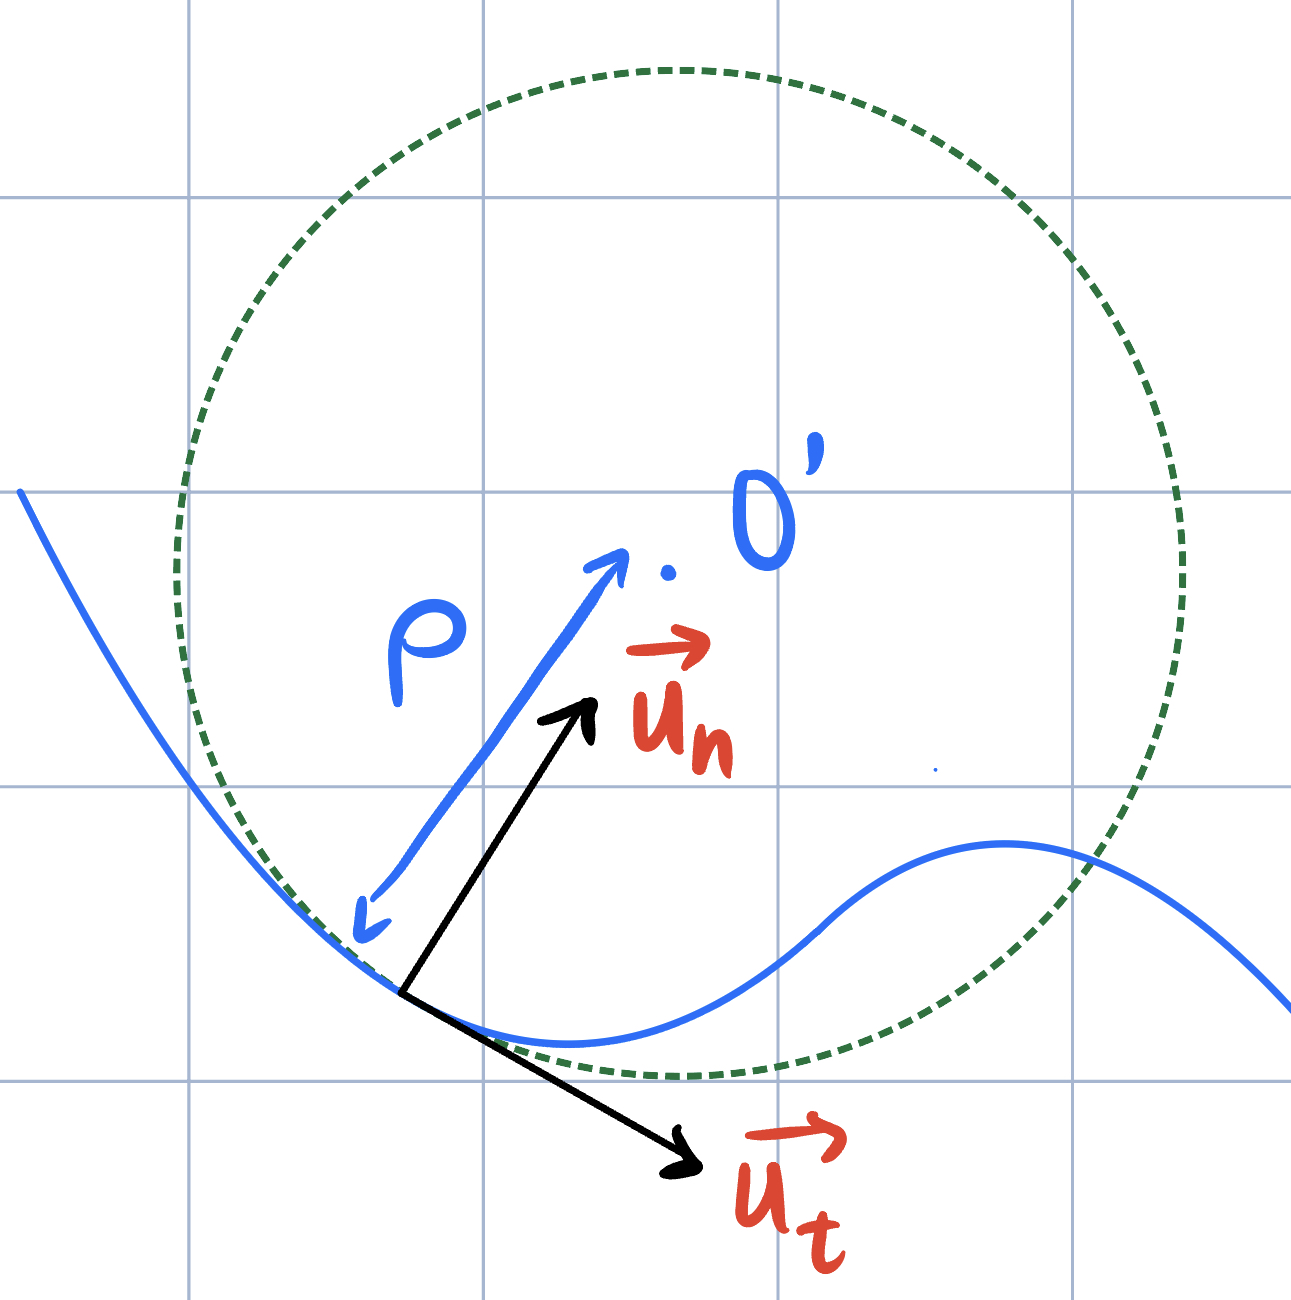
\includegraphics[scale=0.05]{images/normal_tangential.jpg}
    \end{center}

    $\vec{u}_t$ and $\vec{u}_n$

    $s=s(t)\implies\vec{v}=\dot{s}\vec{u}_t$

    $a_t=\dot{v}=\ddot{s}$

    $a_n=\frac{v^2}{\rho}$

    $a=\sqrt{a_t^2+a_n^2}$
\end{multicols}

\newcolumn 

\heading{Polar Coordinates}

\begin{center}
    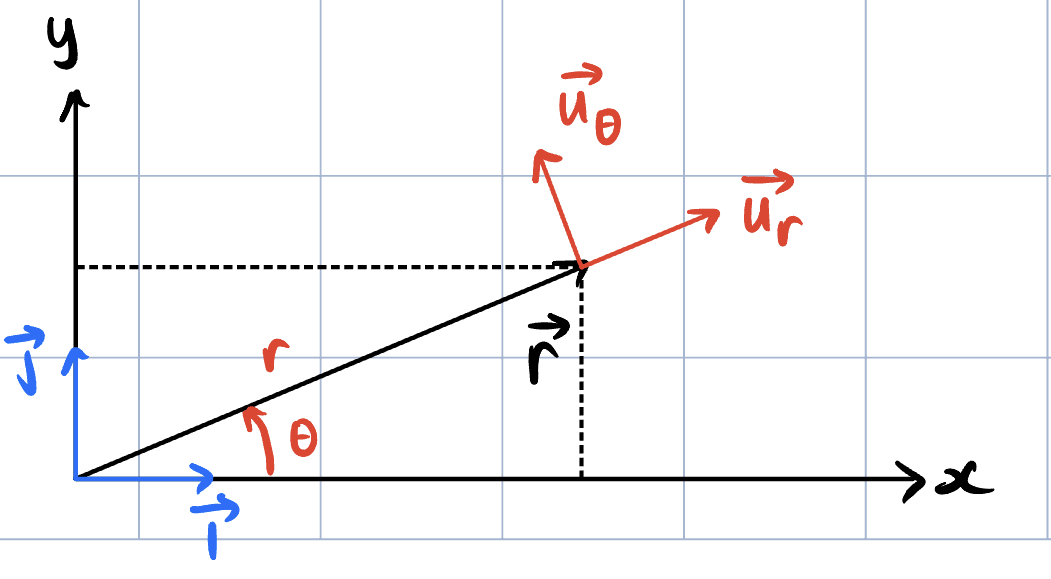
\includegraphics[scale=0.15]{images/polar.jpg}
\end{center}
\begin{align*}
    \vec v&=(\dot r)\vec{u}_r+(r\dot{\theta})\vec{u}_\theta \\
    \vec a&=(\ddot{r}-r\dot{\theta}^2)\vec{u}_r+(r\ddot{\theta}+2\dot{r}\dot{\theta})\vec{u}_\theta
\end{align*}

\heading{Constrained Motion}

\begin{enumerate}[itemsep=0pt,topsep=0pt]
    \item Set datums.
    \item Write rope lengths and positions $s$.
    \item Differentiate to find $v$.
\end{enumerate}

\heading{Polar $\Leftrightarrow$ Normal-Tangential Conversion}

$\psi$: angle from $\vec u_r$ to $\vec u_t$. Positive if CCW, negative if CW.

\begin{center}
    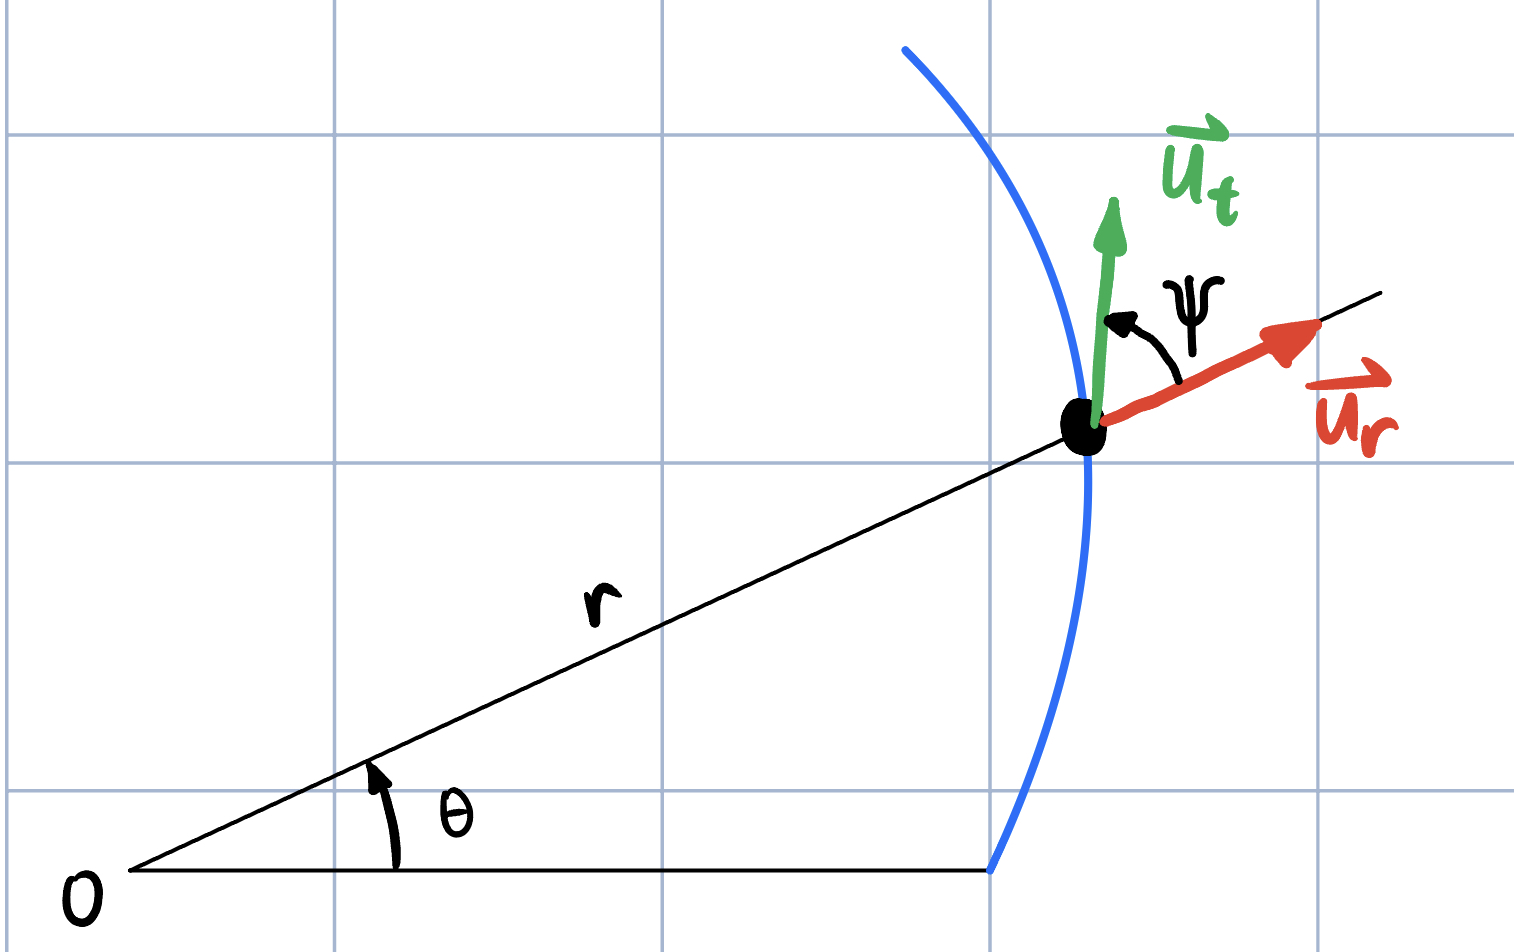
\includegraphics[scale=0.1]{images/polar_nt_conversion.jpg}
\end{center}
\[\tan\psi=\frac{r}{dr/d\theta}\]

Unify coordinate system:
\begin{enumerate}[itemsep=0pt]
    \item Analyze geometry
    \item Convert unit vectors 
    \item Convert forces
\end{enumerate}

\heading{Relative motion}

\[\vec v_{B/A}=\vec v_B-\vec v_A\]
\[\vec a_{B/A}=\vec a_B-\vec a_A\]

\newcolumn

\sectionheading{Work and Energy}

\heading{Energy}

\begin{tabular}{@{}ll}
    Kinetic & $T=\frac{mv^2}{2}$ \\
    Potential & $V^{(g)}=mgh \qquad V^{(s)}=\frac{k\Delta x^2}{2}$
\end{tabular}

\heading{Work}
\begin{align*}
    U &= -U_{\text{external}} \\
    U &= \int_1^2 \vec F\cdot\,d\vec{r} \\
    U_{1\rightarrow 2}^{(g)}&=mg(y_1-y_2) \\
    U_{1\rightarrow 2}^{(s)}&=\frac k2(x_1^2-x_2^2)
\end{align*}

\heading{Work-Energy Principle}
\begin{align*}
    \Delta T&=U_{1\rightarrow 2} \quad (\text{Change in KE = external work}) \\
    T_2 &= T_1+U_{1\rightarrow 2} \\
    T_2+V_2 &= T_1+V_1+U_{1\rightarrow 2}^{(\text{non-cons})}
\end{align*}
{\small \[\frac 12mv_2^2+mgy_2+\frac 12k\Delta_{x_2}^2=\frac 12mv_1^2+mgy_1+\frac 12k\Delta_{x,1}^2+U_{1\rightarrow 2}^{(\text{non-cons})}\]}

\heading{Momentum and Impulse}

\[\vec L=m\vec v \qquad \vec I=\int_{t_1}^{t_2}\vec F\,dt\]

Impulse-Momentum Principle:
\[\Delta \vec L=\vec I_{1\rightarrow 2} \iff \vec L_2=\vec L_1+\vec I_{1\rightarrow 2}\]

Closed system:
\[\sum m_i\vec v_{i,2}=\sum m_i\vec v_{i,1}\]

\end{multicols*}

\end{document}